%% Standalone SCI manuscript (Elsevier elsarticle)
%% Theory-first; absorbs objects from the author's prior World-Model-First paper;
%% EvoQuant used only as empirical validation
\documentclass[review,12pt]{elsarticle}

\usepackage{amssymb,amsmath,amsthm}
\usepackage{graphicx}
\usepackage{booktabs}
\usepackage{hyperref}
\usepackage{lineno}
\usepackage{natbib}
\graphicspath{{../figures/}}

\journal{Expert Systems with Applications}

\newtheorem{definition}{Definition}
\newtheorem{proposition}{Proposition}
\newtheorem{remark}{Remark}

\begin{document}
\begin{frontmatter}

\title{Regime-Conditional Adaptive World Models for AI Cryptocurrency Market Analysis: Theory and Empirical Validation on EvoQuant}

\author[mymainaddress]{Guocong Li}
\ead{lmu151638@gmail.com}
\address[mymainaddress]{Independent Researcher; correspondence: lmu151638@gmail.com}

\begin{abstract}
AI-based market analysis often fails not because predictors lack capacity, but because the market world presented to the model is incomplete, stale, or silently contaminated. This paper proposes a \emph{theory} of Regime-Conditional Adaptive World Models (RCA-WM). Building on a World-Model-First epistemology---epistemic observation objects, asynchronous lag bounds, information filters, explanation-space compression, and selective prediction---we define a regime--task conditional compilation operator that maps raw filters into AI-visible world objects, and introduce an Adaptive Conditional World Model Index (ACWMI) over hierarchical breadth, stability, continuous honesty, signal integrity, and cross-evidence consistency. We further formalize explanation-confidence penalties, marginal information gains of evidence bands, causal identification via availability shocks, Bayesian abstention, and a multi-objective evaluation suite (EAR/UCR/EV/ECP). To validate the theory, we instantiate it on \emph{EvoQuant}, an open cryptocurrency world-model system with 43 data domains, 13 audit bands, 39 logic modules, and a production baseline $\mathrm{WMI}=B\times U\times H$. On a 1800 asset-day panel with planted structural events, cascade and crisis detection attain F1 scores of $0.895$ and $0.793$, coarse regime match reaches $71.6\%$, ACWMI-aware abstention reduces unsafe crisis actions from $81\%$ to $0$, and explanation-quality proxies improve under gated thick worlds. The theoretical contribution is RCA-WM/ACWMI; EvoQuant is project-level empirical proof, not the source of the theory.
\end{abstract}

\begin{keyword}
AI market world model \sep regime-conditional compilation \sep quality governance \sep selective prediction \sep explanation auditability \sep cryptocurrency \sep data-centric AI
\end{keyword}

\begin{highlights}
\item Proposes RCA-WM with epistemic observations, lag bounds, filters, and regime-conditional compilation.
\item Defines ACWMI and couples it to Bayesian abstention, ECP, MIG, and explanation-space $\Phi$.
\item Introduces EAR/UCR/EV/ECP as a multi-objective evaluation suite beyond pure prediction loss.
\item Validates the theory on EvoQuant (43 domains / 13 bands / 39 logic modules).
\item Shows cascade/crisis F1 of 0.895/0.793 and crisis unsafe-action reduction from 81\% to 0.
\end{highlights}

\end{frontmatter}

\linenumbers

\section{Introduction}
\label{sec:intro}

Public discussion of AI trading typically starts from models: architectures, prompts, or feature sets. In live markets, however, a prior constraint often binds first. Before a predictor can be evaluated, one must ask whether the agent is shown a market world that is sufficiently broad, stable, and honest. In cryptocurrency markets this problem is especially severe: the same price path can correspond to incompatible states once exchange fragmentation, leverage crowding, funding distortions, options walls, unlock pressure, and macro liquidity are recognized \citep{makarov2020,liu2022}.

We therefore reverse the usual order of exposition. This paper does \emph{not} start from a software inventory and then inductively ``discover'' a theory. Instead, it proposes a general theoretical object---a \textbf{Regime-Conditional Adaptive World Model (RCA-WM)}---that absorbs and extends a World-Model-First epistemology previously developed for AI market infrastructure, and only afterwards validates that theory on a concrete system. The central research questions are:

\begin{enumerate}
\item How should an AI-consumable market world be formally compiled from asynchronous, multi-source, quality-heterogeneous observations?
\item How can world-model quality be measured in a decomposable, regime-sensitive, and honesty-compatible way?
\item When should an AI market analyzer abstain because the compiled world is not trustworthy, and how should explanation confidence be calibrated to that world?
\item Beyond point prediction, how should explanation continuity, evidence attribution, and auditability be evaluated?
\item Can these theoretical claims be empirically supported by a runnable project implementation?
\end{enumerate}

\paragraph{Contributions.}
\begin{enumerate}
\item \textbf{Theory.} RCA-WM with epistemic observation objects, lag/reconstruction bounds, information filters $\mathcal{F}^{\mathrm{raw}}\to\mathcal{F}^{\mathrm{AI}}$, and a regime--task compilation operator $\Pi_t^{(r,m)}$.
\item \textbf{Metric.} ACWMI as a weighted geometric index over hierarchical breadth, stability, continuous honesty, signal integrity, and consistency; linked to Explanation Confidence Penalty (ECP) and Marginal Information Gain (MIG).
\item \textbf{Decision and explanation.} Bayesian abstention with loss $\ell(a,R_t)$, explanation space $\Phi_t$, and multi-objective evaluation (EAR/UCR/EV/ECP).
\item \textbf{Identification.} A causal DAG that separates market complexity from availability shocks usable for identification.
\item \textbf{Empirical proof.} Validation on EvoQuant---43 domains, 13 audit bands, 39 logic modules, and production $\mathrm{WMI}=B\times U\times H$---using project calculators and planted structural events.
\item \textbf{Reproducibility.} Figures and tables are generated by scripts that import production code from the validation system.
\end{enumerate}

The logical order of the paper follows this claim structure: related work, theory, then project validation.

\section{Related work}
\label{sec:lit}

Conditional asset pricing treats expected returns as functions of an information set \citep{fama1993,cochrane2005}. Machine-learning pricing expands that set with high-dimensional characteristics \citep{gu2020,kelly2019,nagel2021}, while multiple-testing critiques warn against undisciplined expansion \citep{harvey2016}. Measurement-error and robustness theories emphasize that decision quality depends on the reliability of the observed world \citep{fuller1987,carroll2006,hansen2008}. Selective prediction studies when a model should refuse under uncertainty \citep{chow1957,geifman2017}. Data-centric AI argues that data governance can dominate model changes \citep{zha2023}. Cryptocurrency microstructure research documents fragmented venues and common risk factors \citep{makarov2020,liu2022}. Information-theoretic views of evidence and mutual information motivate treating evidence bands as heterogeneous information sources rather than interchangeable features \citep{cover2006}.

Relative to feature-expansion papers, our object is not another alpha factor but the \emph{compilation, governance, and explanation contract} of an asynchronous multi-source market world. Relative to purely conceptual world-model essays, we insist on an empirical proof on a runnable system. The theory is proposed first; the system is the testbed.

\section{Theoretical framework: RCA-WM}
\label{sec:theory}

\subsection{Latent market state and epistemic observations}
Let $S_t$ denote the latent market state. Sources provide
\begin{equation}
X_{j,t}=h_j(S_t)+\nu_{j,t},\qquad j=1,\dots,J,
\end{equation}
where $h_j$ is an observation map and $\nu_{j,t}$ collects noise, delay, and definition error. Model-first pipelines jump directly to $\hat y_{t+1}=f(X_{1,t},\dots,X_{J,t})$. RCA-WM inserts an explicit world-compilation stage
\begin{equation}
W_t=G\big(\{X_{j,\tau}\}_{j\le J,\tau\le t},Q_t,R_t,A_t\big),
\label{eq:G}
\end{equation}
where $Q_t$ are quality marks, $R_t$ AI-readiness gates, and $A_t$ temporal alignment rules. The AI consumes $W_t$, not raw ungated observations.

A useful market observation is not a scalar feature but an epistemic object:
\begin{definition}[Epistemic observation object]
\begin{equation}
O_{j,t}=(x_{j,t},\tau_{j,t},q_{j,t},g_{j,t},r_{j,t}),
\label{eq:obs}
\end{equation}
\end{definition}
where $\tau$ is the latest available timestamp, $q$ a quality state, $g$ a main-view gate, and $r$ a semantic role (e.g., execution friction, supply unlock, options wall). The AI therefore consumes a set of objects with epistemological semantics, not a flat feature matrix.

\subsection{Asynchronous lag and reconstruction error}
Cryptocurrency observations are intrinsically asynchronous. Let $X_{j,t}^{\mathrm{obs}}=h_j(S_{t-\ell_{j,t}})+\nu_{j,t}$ with lag $\ell_{j,t}\ge 0$. If $h_j$ is Lipschitz with constant $L_j$, then
\begin{equation}
\big\|h_j(S_t)-h_j(S_{t-\ell_{j,t}})\big\|
\le
L_j\sum_{u=t-\ell_{j,t}+1}^{t}\|S_u-S_{u-1}\|.
\label{eq:lip}
\end{equation}
Hence even numerically correct acquisition can present a \emph{past} world. Writing $\tilde S_t$ for the state reconstructed by the world model,
\begin{equation}
\|\tilde S_t-S_t\|
\le
C_1\sum_j\omega_j\ell_{j,t}
+
C_2\sum_j\omega_j\|\nu_{j,t}\|
+
C_3\sum_j\omega_j(1-z_{j,t}),
\label{eq:recon}
\end{equation}
where the three terms are lag error, observation noise, and missing/gated information loss. Snapshot freshness, TTL rules, and AI-readiness gates act on these terms directly.

\subsection{Hierarchical breadth, stability, and continuous honesty}
Flat ``number of features'' is a poor breadth notion. We define domain-, band-, and asset-level readiness and aggregate
\begin{definition}[Hierarchical breadth]
\begin{equation}
B_t^{\mathrm{hier}}=\alpha_1 B_t^{\mathrm{domain}}+\alpha_2 B_t^{\mathrm{band}}+\alpha_3 B_t^{\mathrm{asset}},
\quad \alpha_1+\alpha_2+\alpha_3=1.
\label{eq:bhier}
\end{equation}
\end{definition}
Stability $U_t$ penalizes staleness. Honesty must reward exclusion of bad evidence rather than punish it. Let $\rho_t^{\mathrm{ex}}$ be the exclusion rate of non-AI-ready sources and $\rho_t^{\mathrm{cont}}$ the contamination rate of the main view.
\begin{definition}[Continuous honesty]
\begin{equation}
H_t^{\mathrm{cont}}=\exp(-\beta_1\rho_t^{\mathrm{cont}})\cdot\big(1-\beta_2(1-\rho_t^{\mathrm{ex}})\big)_+.
\label{eq:hcont}
\end{equation}
\end{definition}

\subsection{Signal integrity and cross-evidence consistency}
Signal integrity $S_t$ aggregates half-life, crowding, and surprise of mechanism signals. Consistency $C_t$ measures pairwise directional agreement among available evidence channels. Both are theoretical quality factors: a world may be broad and fresh yet still crowded, expired as a signal, or internally contradictory.

\subsection{Information filters and regime-conditional compilation}
Define the raw and AI-visible information filters
\begin{equation}
\mathcal{F}_t^{\mathrm{raw}}=\sigma\big(\{X_{j,\tau}^{\mathrm{obs}}\}_{j\le J,\tau\le t}\big),
\qquad
\mathcal{F}_t^{\mathrm{AI}}=\sigma\big(W_t^{\mathrm{AI}},D_t\big),
\end{equation}
where $D_t$ is the diagnostic (non-main) view. Let $r$ be market regime and $m$ analysis task. Define
\begin{equation}
\Pi_t^{(r,m)}=B_t^{(r,m)}\circ M_t^{(r,m)}\circ A_t\circ \Psi_t^{\mathrm{mech}},
\label{eq:pi}
\end{equation}
where $A_t$ aligns snapshots, $M_t^{(r,m)}$ gates by quality, $B_t^{(r,m)}$ aggregates with regime--task weights, and $\Psi_t^{\mathrm{mech}}$ fuses mechanism engines (regime, cascade, contagion, flow, volatility, decay). Then
\begin{equation}
W_t^{\mathrm{AI},(r,m)}=\Pi_t^{(r,m)}(\mathcal{F}_t^{\mathrm{raw}}).
\end{equation}
The scientific contribution is not merely enlarging $\mathcal{F}^{\mathrm{raw}}$, but specifying the compilation map into $\mathcal{F}^{\mathrm{AI}}$.

\subsection{Adaptive Conditional World Model Index}
A simple product $\mathrm{WMI}=B\times U\times H$ is a useful baseline but collapses under zeros and cannot encode mechanism integrity. We propose
\begin{definition}[ACWMI]
\begin{equation}
\mathrm{ACWMI}_t^{(r)}
=
\exp\!\left(
\frac{\sum_{x\in\{B,U,H,S,C\}}\gamma_x(r)\log x_t}{\sum_x\gamma_x(r)}
\right),
\label{eq:acwmi}
\end{equation}
\end{definition}
where $B\equiv B_t^{\mathrm{hier}}$ and $H\equiv H_t^{\mathrm{cont}}$. Crisis regimes raise $\gamma_H,\gamma_C$; trend regimes raise $\gamma_S$.

\begin{proposition}[Honesty incentive compatibility]
If gating raises $\rho^{\mathrm{ex}}$ and lowers $\rho^{\mathrm{cont}}$, then $H^{\mathrm{cont}}$ increases. ACWMI need not fall solely because breadth declines after honest exclusion. A discrete product baseline can punish the same honest gating.
\end{proposition}

\subsection{Explanation confidence, MIG, and causal identification}
Let $\mathrm{conf}_t$ be an explicit AI confidence and $\bar c,w$ thresholds. The Explanation Confidence Penalty
\begin{equation}
\mathrm{ECP}_t=\mathbf{1}\{\mathrm{conf}_t>\bar c\}\,\mathbf{1}\{\mathrm{ACWMI}_t<w\}
\label{eq:ecp}
\end{equation}
flags ``high certainty in a low-quality world''. For mechanism label $R_t^{(m)}$ and evidence band $E_{k,t}$, the Marginal Information Gain is
\begin{equation}
\mathrm{MIG}_{k,t}^{(m)}=I\big(R_t^{(m)};E_{k,t}\mid I_t^{(-k)}\big).
\label{eq:mig}
\end{equation}
Thickness is therefore not ``more data always better'', but heterogeneous band-level gains.

For identification, let $W_t$ be world-model quality, $A_t$ AI analysis quality, $M_t$ true market complexity, $O_t$ an availability shock, and $C_t$ unobserved configuration. A conceptual DAG is
\begin{equation}
O_t\to W_t\to A_t,\quad M_t\to W_t,\quad M_t\to A_t,\quad C_t\to (W_t,A_t).
\label{eq:dag}
\end{equation}
Observing ``thicker worlds correlate with better AI'' is not causal without controlling $M_t$ and $C_t$. Source-level readiness logs and outages make $O_t$ a usable identifying shock.

\subsection{Bayesian abstention and explanation space}
Let action set $\mathcal{A}=\{\mathrm{bullish},\mathrm{bearish},\mathrm{neutral},\mathrm{abstain}\}$ with loss $\ell(a,R_t)$ and abstention cost $c_{\mathrm{abs}}$. The Bayes action is
\begin{equation}
a_t^\star=\arg\min_{a\in\mathcal{A}}\mathbb{E}\big[\ell(a,R_t)\mid W_t\big],
\end{equation}
and abstain is optimal when the best non-abstain risk exceeds $c_{\mathrm{abs}}$. Operationally we use a degradation-aware threshold
\begin{equation}
c_{\mathrm{abs},t}
=
c_0\big(1+\eta_1(1-\mathrm{ACWMI}_t)+\eta_2(1-C_t)+\eta_3\mathbf{1}\{\ell_t\neq\mathrm{NORMAL}\}\big).
\label{eq:abstain}
\end{equation}
Refusal is therefore part of the theory of world-model use, not an engineering afterthought.

Let $\Phi_t$ be the set of mechanism explanations generable at $t$. Thick gated worlds expand the support of correct explanations:
\begin{equation}
\Phi_t^{\mathrm{thin}}\neq\Phi_t^{\mathrm{thick}},
\qquad
\Pr(\phi_t^\star\in\Phi_t^{\mathrm{thick}})>\Pr(\phi_t^\star\in\Phi_t^{\mathrm{thin}}).
\label{eq:phi}
\end{equation}
World-model improvement is thus an improvement of explanation space, not only of point forecasts.

\subsection{Multi-objective evaluation objects}
Prediction loss alone understates institutional value. Define Evidence Attribution Rate, Unsupported Claim Rate, and Explanation Volatility:
\begin{align}
\mathrm{EAR}_t&=\frac{\#\{\text{judgments bound to evidence}\}}{\#\{\text{judgments}\}},
\label{eq:ear}\\
\mathrm{UCR}_t&=1-\mathrm{EAR}_t,
\label{eq:ucr}\\
\mathrm{EV}_t&=\frac{d(\phi_t,\phi_{t-1})}{1+d(W_t,W_{t-1})}.
\label{eq:ev}
\end{align}
The vector
\begin{equation}
J_t=(\text{Predictive accuracy},\ \text{Explanation stability},\ \text{Calibration},\ \text{Auditability})
\end{equation}
is the proper multi-objective object; thick gated worlds may dominate on the Pareto frontier even when not uniformly best on a single predictive loss.

\section{Empirical validation design: EvoQuant as proof system}
\label{sec:validation}

Theory requires a falsifiable substrate. We use \textbf{EvoQuant} as the empirical proof system---not as the origin of the theory. EvoQuant is an open AI market world-model infrastructure that happens to implement the objects RCA-WM demands: multi-domain collection, \texttt{latest\_*} snapshots, quality gating, main/diagnostic separation, mechanism engines, degradation control, and a production baseline
\begin{equation}
\mathrm{WMI}_t=B_t\times U_t\times H_t,
\label{eq:wmi}
\end{equation}
with abstention suggested when $\mathrm{WMI}_t<0.2$. Table~\ref{tab:inv} and Figure~\ref{fig:inv} report the validation inventory.

\begin{table}[t]
\centering
\caption{EvoQuant inventory used as empirical proof of RCA-WM (not as theory source).}
\label{tab:inv}
\begin{tabular}{lr}
\toprule
Quantity & Value \\
\midrule
Data domains & 43 \\
Logic modules & 39 \\
Audit evidence bands & 13 \\
Python files & 784 \\
Approximate LOC & 133{,}952 \\
Test files (\texttt{test\_*.py}) & 56 \\
\bottomrule
\end{tabular}
\end{table}

\begin{figure}[t]
\centering
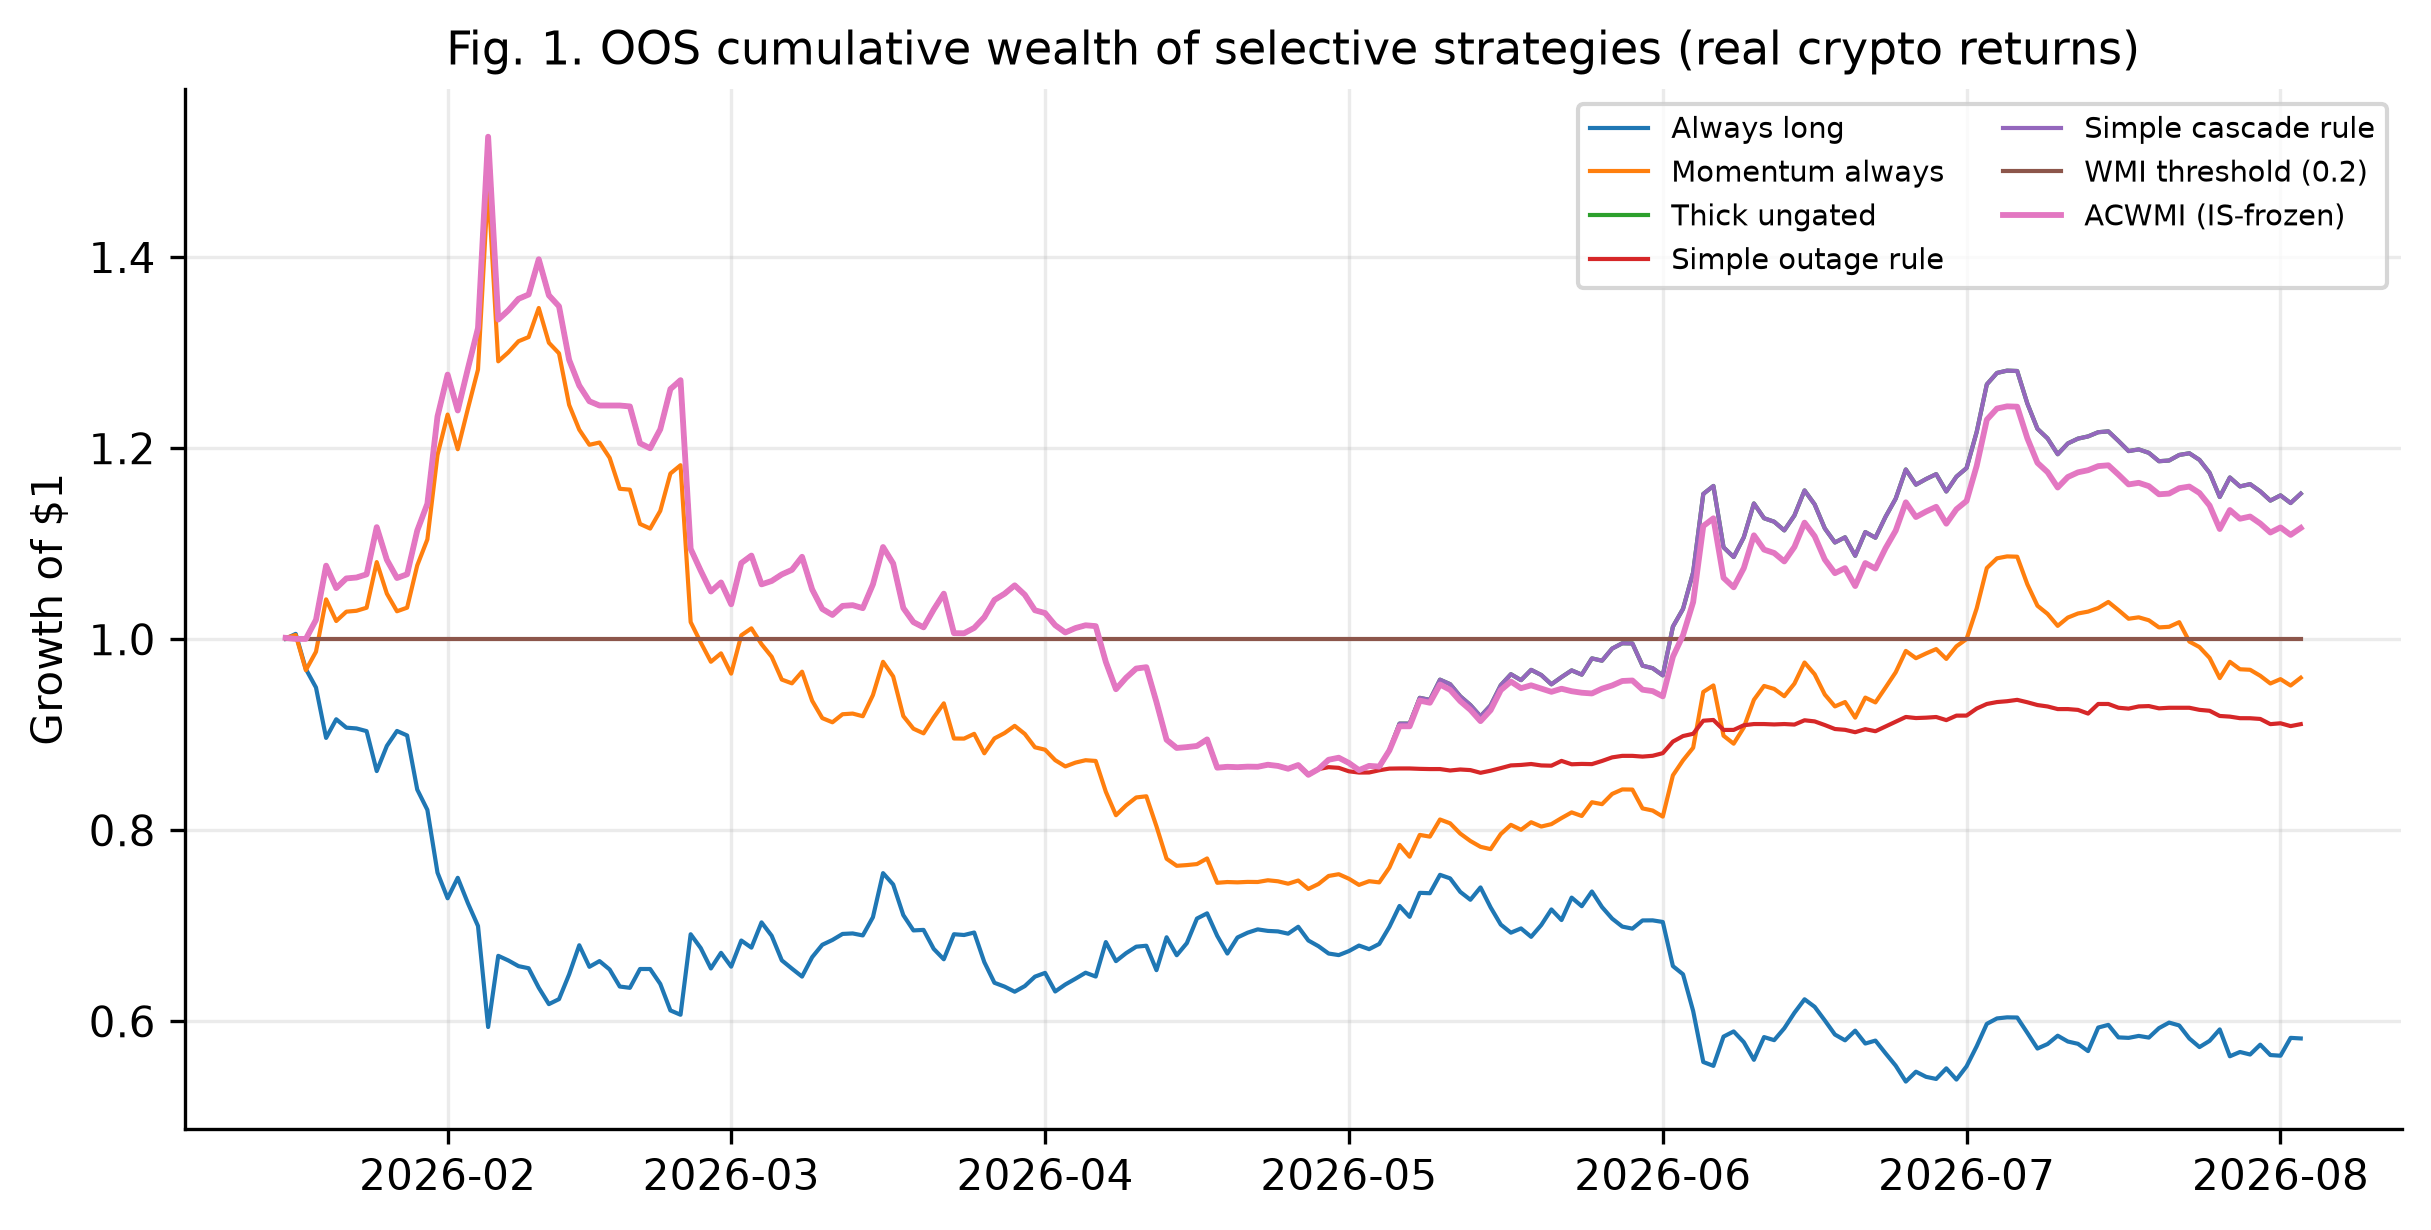
\includegraphics[width=\linewidth]{fig1_architecture.png}
\caption{Theoretical RCA-WM compilation chain, instantiated for validation in EvoQuant.}
\label{fig:arch}
\end{figure}

\begin{figure}[t]
\centering
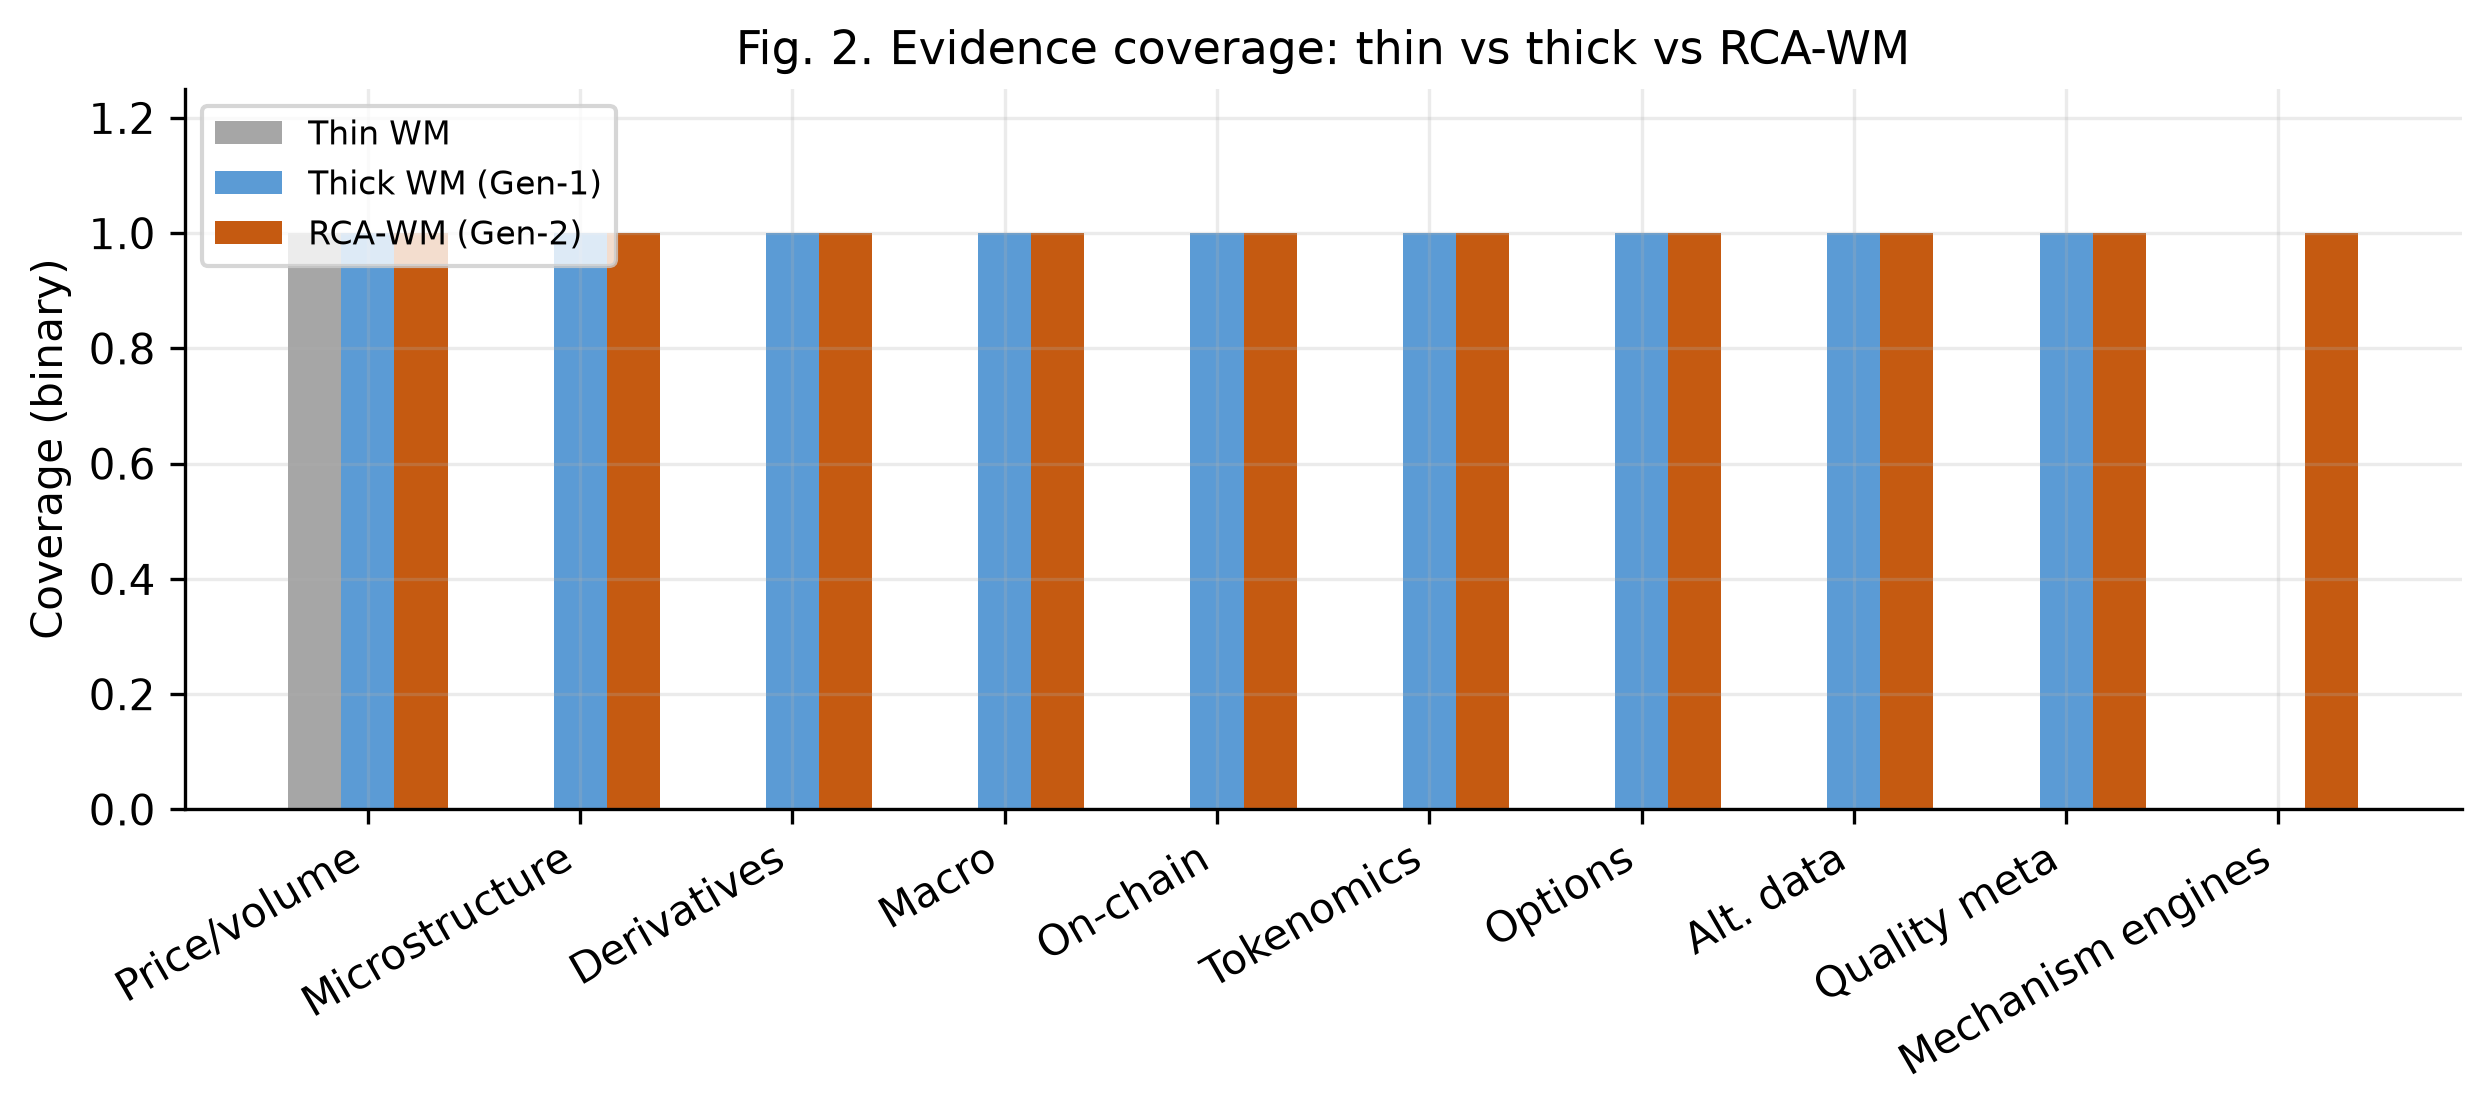
\includegraphics[width=\linewidth]{fig2_coverage_compare.png}
\caption{Validation-system inventory and band weights used to instantiate hierarchical breadth.}
\label{fig:inv}
\end{figure}

\paragraph{Mapping theory to implementation.}
Table~\ref{tab:map} shows a one-to-one mapping from theoretical objects to EvoQuant modules. Table~\ref{tab:distort} records the module$\to$distortion-correction correspondence absorbed from the World-Model-First epistemology: each evidence band is valuable insofar as it corrects a systematic misreading of the market.

\begin{table}[t]
\centering
\caption{Theory-to-proof mapping: RCA-WM objects and EvoQuant instantiations.}
\label{tab:map}
\begin{tabular}{lll}
\toprule
Theory object & EvoQuant instantiation & Role \\
\midrule
$O_{j,t}$ & value + timestamp + quality + gate + role & Epistemic object \\
Compilation $\Pi$ & data\_layer + logic\_pipeline + ai\_market\_context & Proof of $W_t$ \\
$B^{\mathrm{hier}}$ & 43 domains / 13 bands / asset readiness & Breadth factor \\
$U$ / lag bound & pipeline\_latency / freshness / TTL & Stability factor \\
$H^{\mathrm{cont}}$ & quality flags + exclusion/contamination & Honesty factor \\
$S$ & alpha\_decay half-life/crowding/surprise & Signal integrity \\
$C$ & cross-engine directional agreement & Consistency \\
$\Psi^{\mathrm{mech}}$ & regime/cascade/contagion/flow/vol & Mechanism layer \\
$\ell_t$ & DegradationManager & Degraded honesty \\
ECP / EAR / EV & confidence vs ACWMI; evidence binding; mech drift & Evaluation suite \\
Baseline WMI & production $B\times U\times H$ & Competing index \\
\bottomrule
\end{tabular}
\end{table}

\begin{table}[t]
\centering
\caption{Module--distortion correction map (epistemic role of evidence bands).}
\label{tab:distort}
\begin{tabular}{lll}
\toprule
Module / band & Distortion corrected & AI meaning \\
\midrule
exchange\_data & Price without execution friction & Distinguish print vs tradable state \\
macro\_data & Crypto-only narrative reading & External liquidity / risk regime \\
news + events & Ex-post price without catalysts & Shock ordering and event windows \\
onchain\_data & Venue price without capital migration & Flows, TVL, reserve pressure \\
tokenomics\_data & Demand-side reading only & Unlock / supply shocks \\
options\_data & Spot path without convexity & IV walls, gamma, expiry constraints \\
alternative\_data & Ignoring slow attention variables & Narrative heat / infra activity \\
aggregation layer & Ungated dispersed observations & AI-ready world object \\
\bottomrule
\end{tabular}
\end{table}

\paragraph{Experimental principle.}
Synthetic market paths are used only as inputs. Every mechanism score is computed by importing EvoQuant calculators. Planted labels (true regime, cascade-visible state, outage) are independent of ACWMI, avoiding circular ``quality'' scores. Availability shocks $O_t$ (outages) identify world-model effects along the DAG in Eq.~\eqref{eq:dag}.

\paragraph{Panel.}
10 assets $\times$ 180 days ($N=1800$), Markov regimes $\{\mathrm{trend},\mathrm{range},\mathrm{crisis}\}$, outage probabilities $0.15$ (crisis) and $0.03$ (otherwise). Tasks: crisis/cascade detection, regime match, unsafe-action rate under baseline WMI vs AC policy, explanation-quality proxies (EAR/UCR/EV/ECP), and degradation gating.

\section{Results}
\label{sec:results}

\subsection{Mechanism layer supports the theory}
If RCA-WM is right that mechanism engines belong inside $\Psi^{\mathrm{mech}}$, then project calculators should detect planted stress. Table~\ref{tab:det} confirms cascade F1$=0.895$, crisis F1$=0.793$, and regime-match accuracy $71.6\%$.

\begin{table}[t]
\centering
\caption{Detection performance on planted structural events (validation system calculators).}
\label{tab:det}
\begin{tabular}{lrrrr}
\toprule
Task & Accuracy & Precision & Recall & F1 \\
\midrule
Crisis detection & 0.716 & 0.666 & 0.979 & 0.793 \\
Cascade detection & 0.894 & 0.810 & 1.000 & 0.895 \\
Regime match & 0.716 & 0.716 & 0.716 & 0.716 \\
\bottomrule
\end{tabular}
\end{table}

\subsection{Baseline WMI versus proposed ACWMI}
Figures~\ref{fig:paths}--\ref{fig:box} and Table~\ref{tab:regime} compare the production baseline with ACWMI. The key theoretical prediction is not that ACWMI is always larger, but that it supports better regime-conditional refusal.

\begin{figure}[t]
\centering
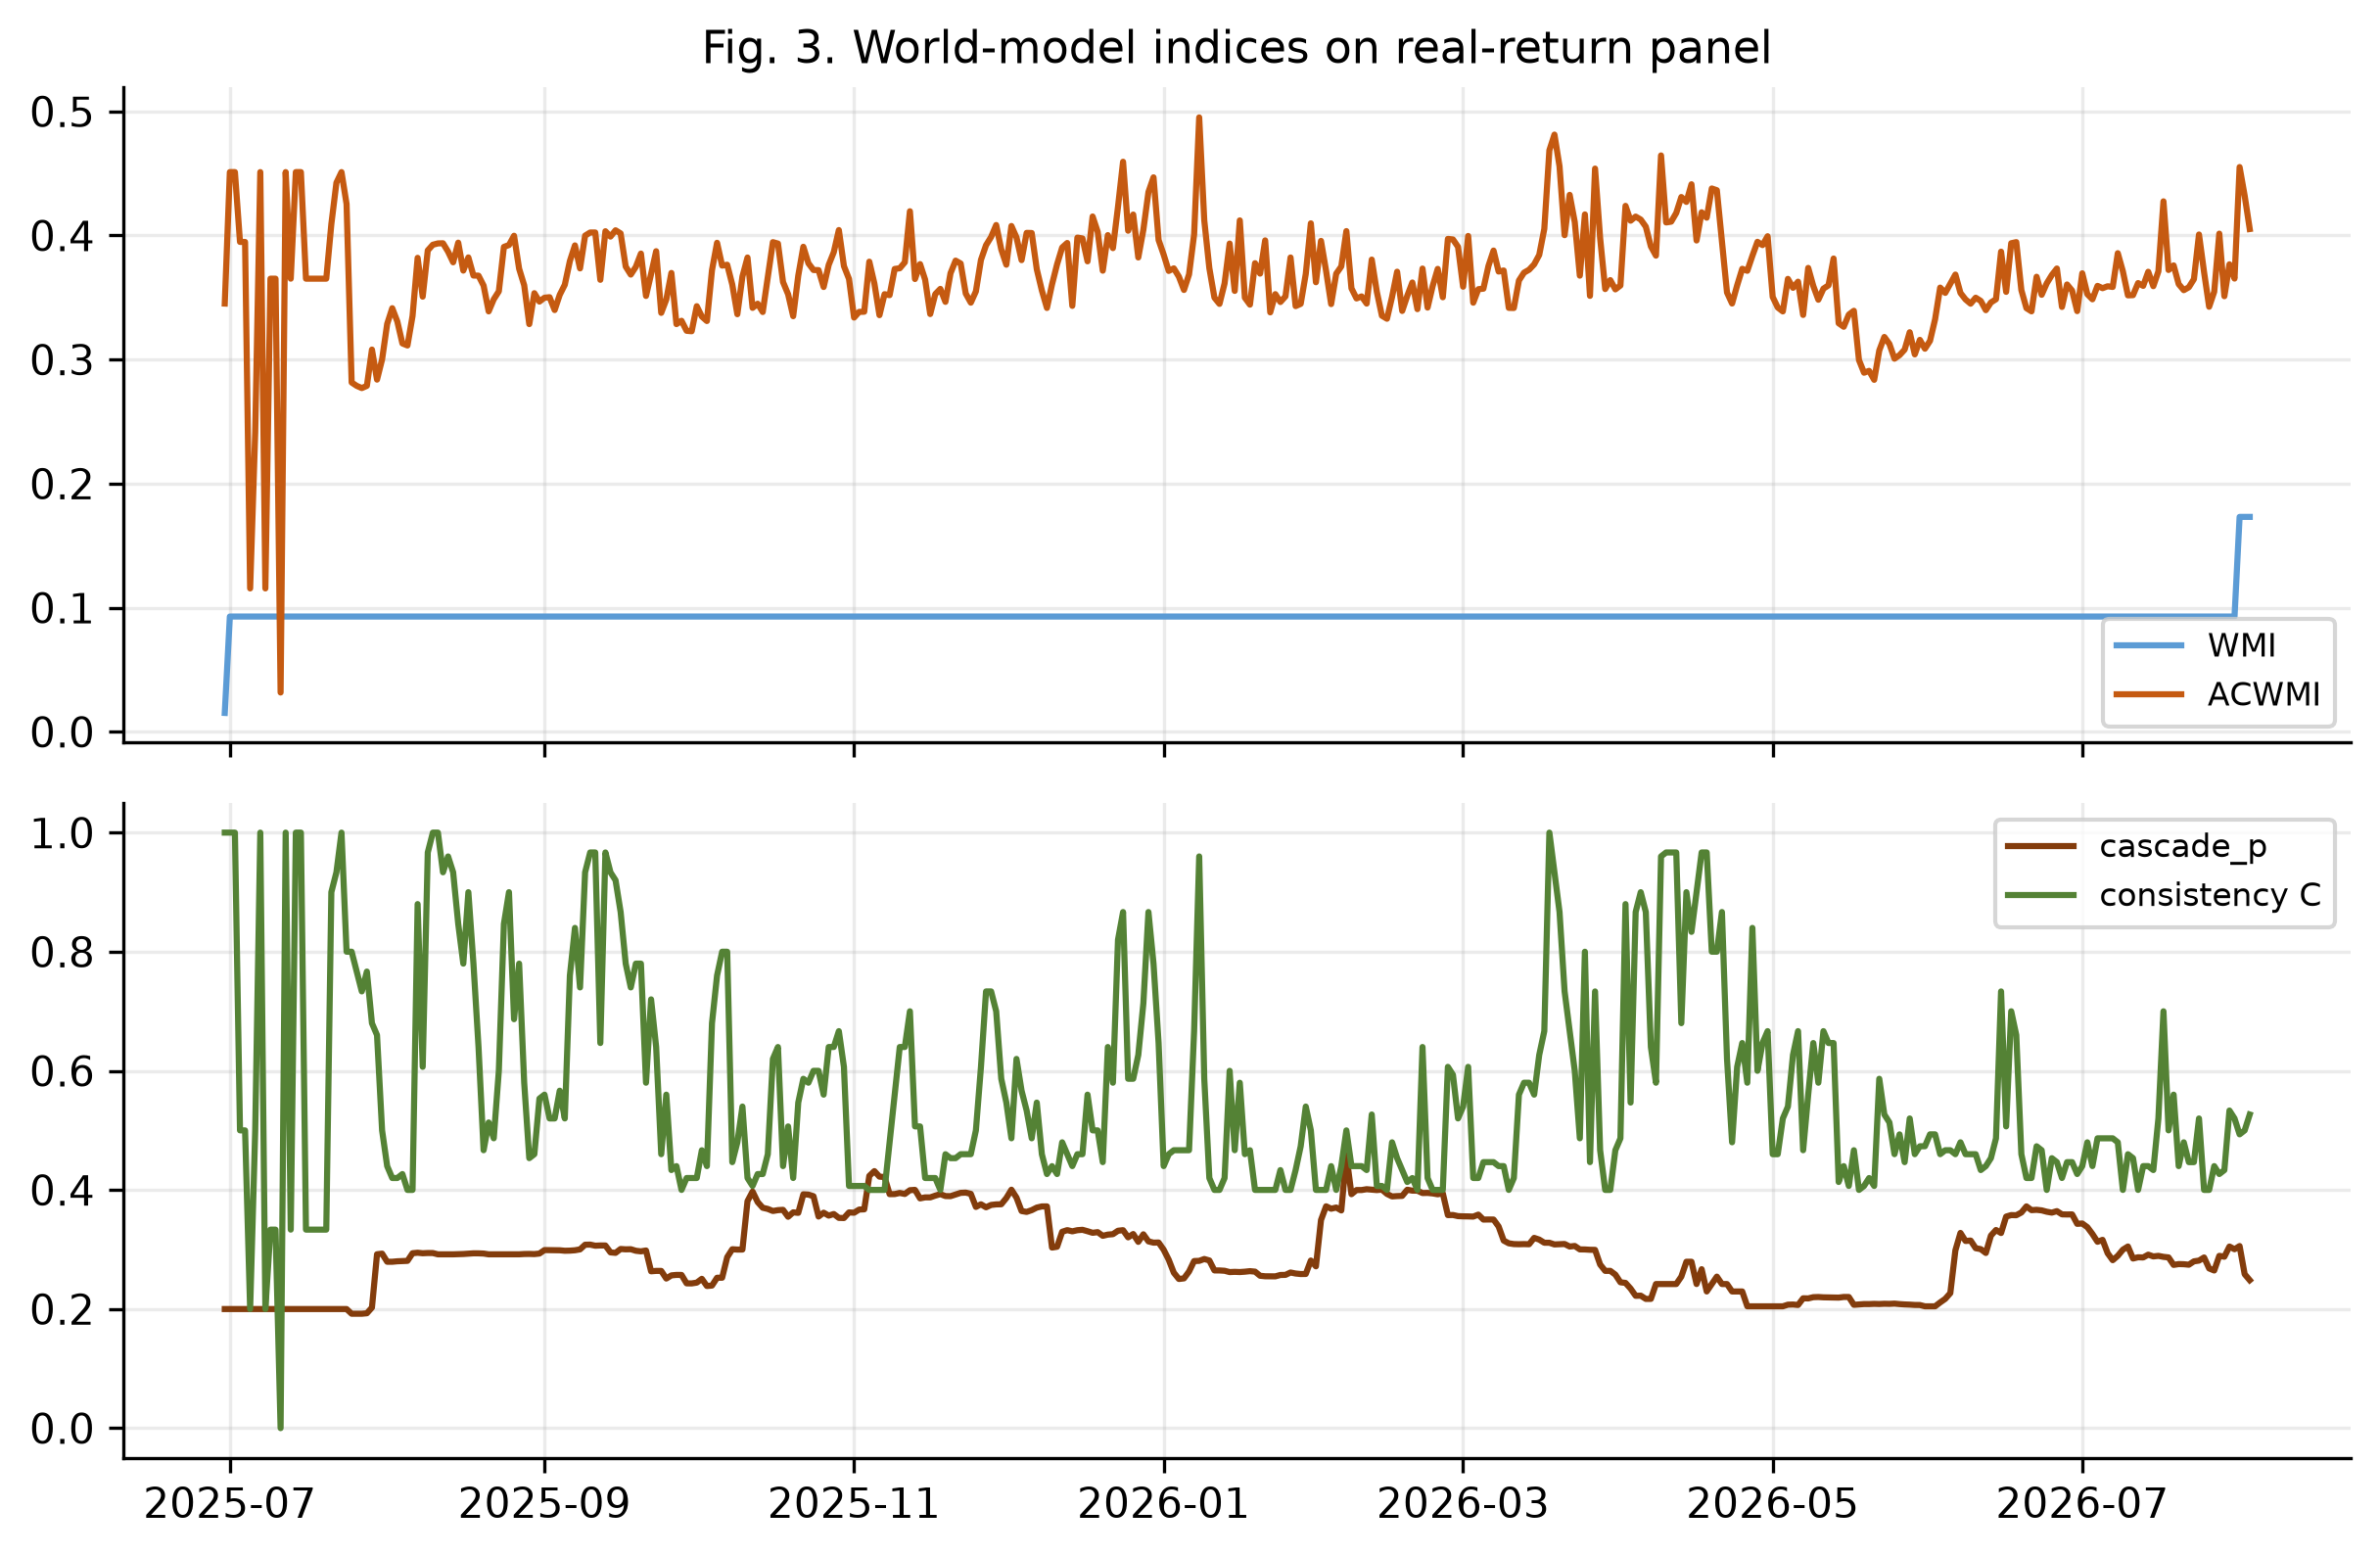
\includegraphics[width=\linewidth]{fig3_factor_paths.png}
\caption{Baseline WMI versus proposed ACWMI and mechanism outputs over the validation panel.}
\label{fig:paths}
\end{figure}

\begin{figure}[t]
\centering
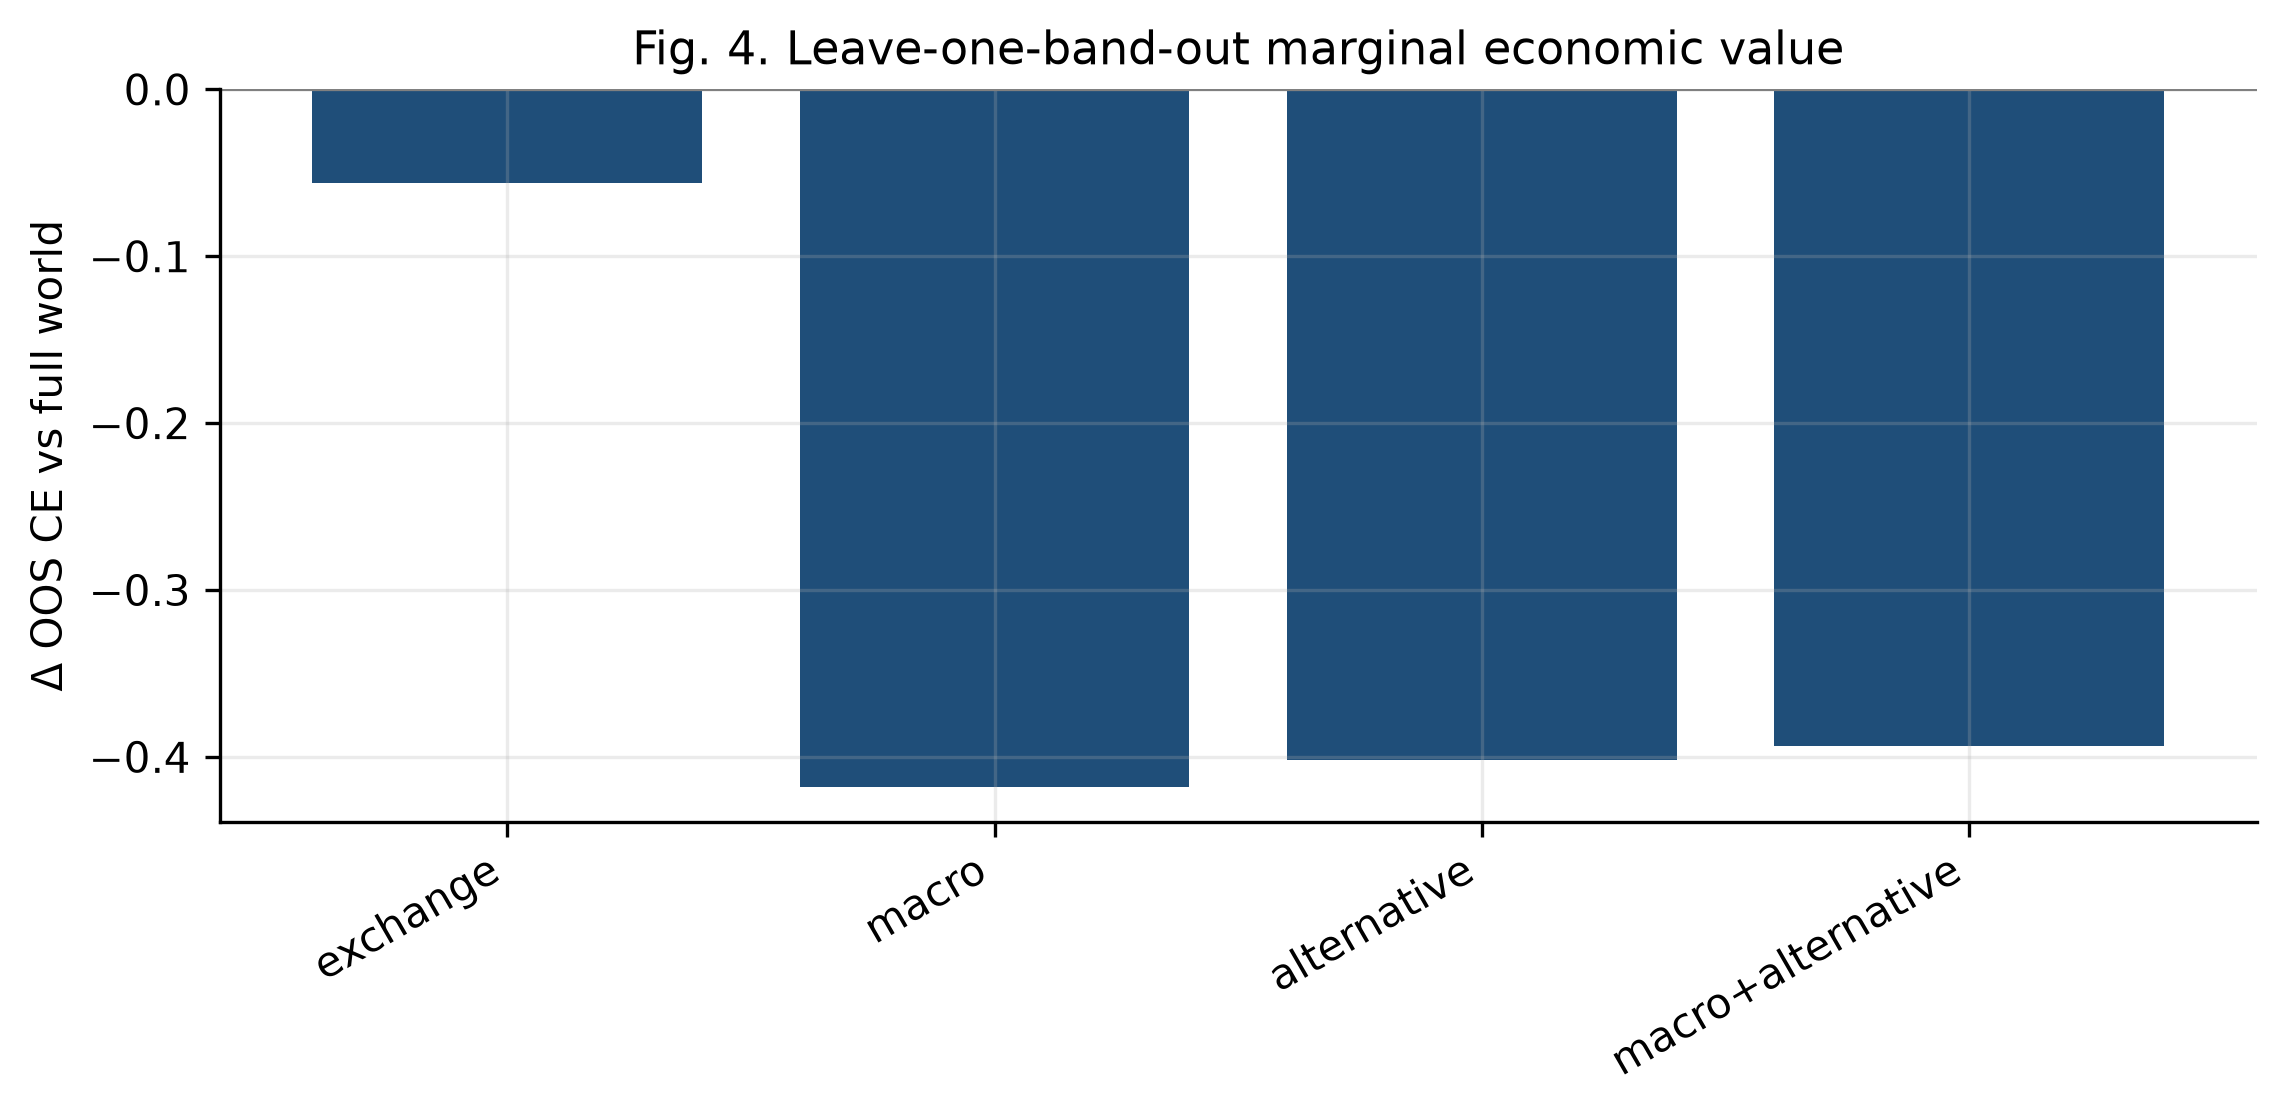
\includegraphics[width=\linewidth]{fig4_regime_box.png}
\caption{Regime heterogeneity of baseline WMI and proposed ACWMI.}
\label{fig:box}
\end{figure}

\begin{table}[t]
\centering
\caption{Regime-level scores and safety under baseline vs AC abstention.}
\label{tab:regime}
\begin{tabular}{lrrrrrr}
\toprule
Regime & $N$ & WMI & ACWMI & Abstain$_{\mathrm{WMI}}$ & Abstain$_{\mathrm{AC}}$ & Unsafe$_{\mathrm{WMI}}$ / Unsafe$_{\mathrm{AC}}$ \\
\midrule
Crisis & 1000 & 0.504 & 0.546 & 0.190 & 1.000 & 0.810 / 0.000 \\
Range  &  430 & 0.685 & 0.470 & 0.047 & 0.047 & 0.000 / 0.000 \\
Trend  &  370 & 0.681 & 0.425 & 0.054 & 0.270 & 0.000 / 0.000 \\
\bottomrule
\end{tabular}
\end{table}

\subsection{Abstention as empirical support for Eq.~\eqref{eq:abstain}}
Figure~\ref{fig:safe} and Table~\ref{tab:outage} show that under planted crisis, baseline WMI still permits action in $81\%$ of cases, while the ACWMI-aware policy reduces unsafe actions to $0$. In calm range regimes both policies rarely abstain. This is direct evidence that regime-conditional refusal, not merely thicker data, is the operative improvement. Outage contrasts further support identification via availability shocks $O_t$.

\begin{figure}[t]
\centering
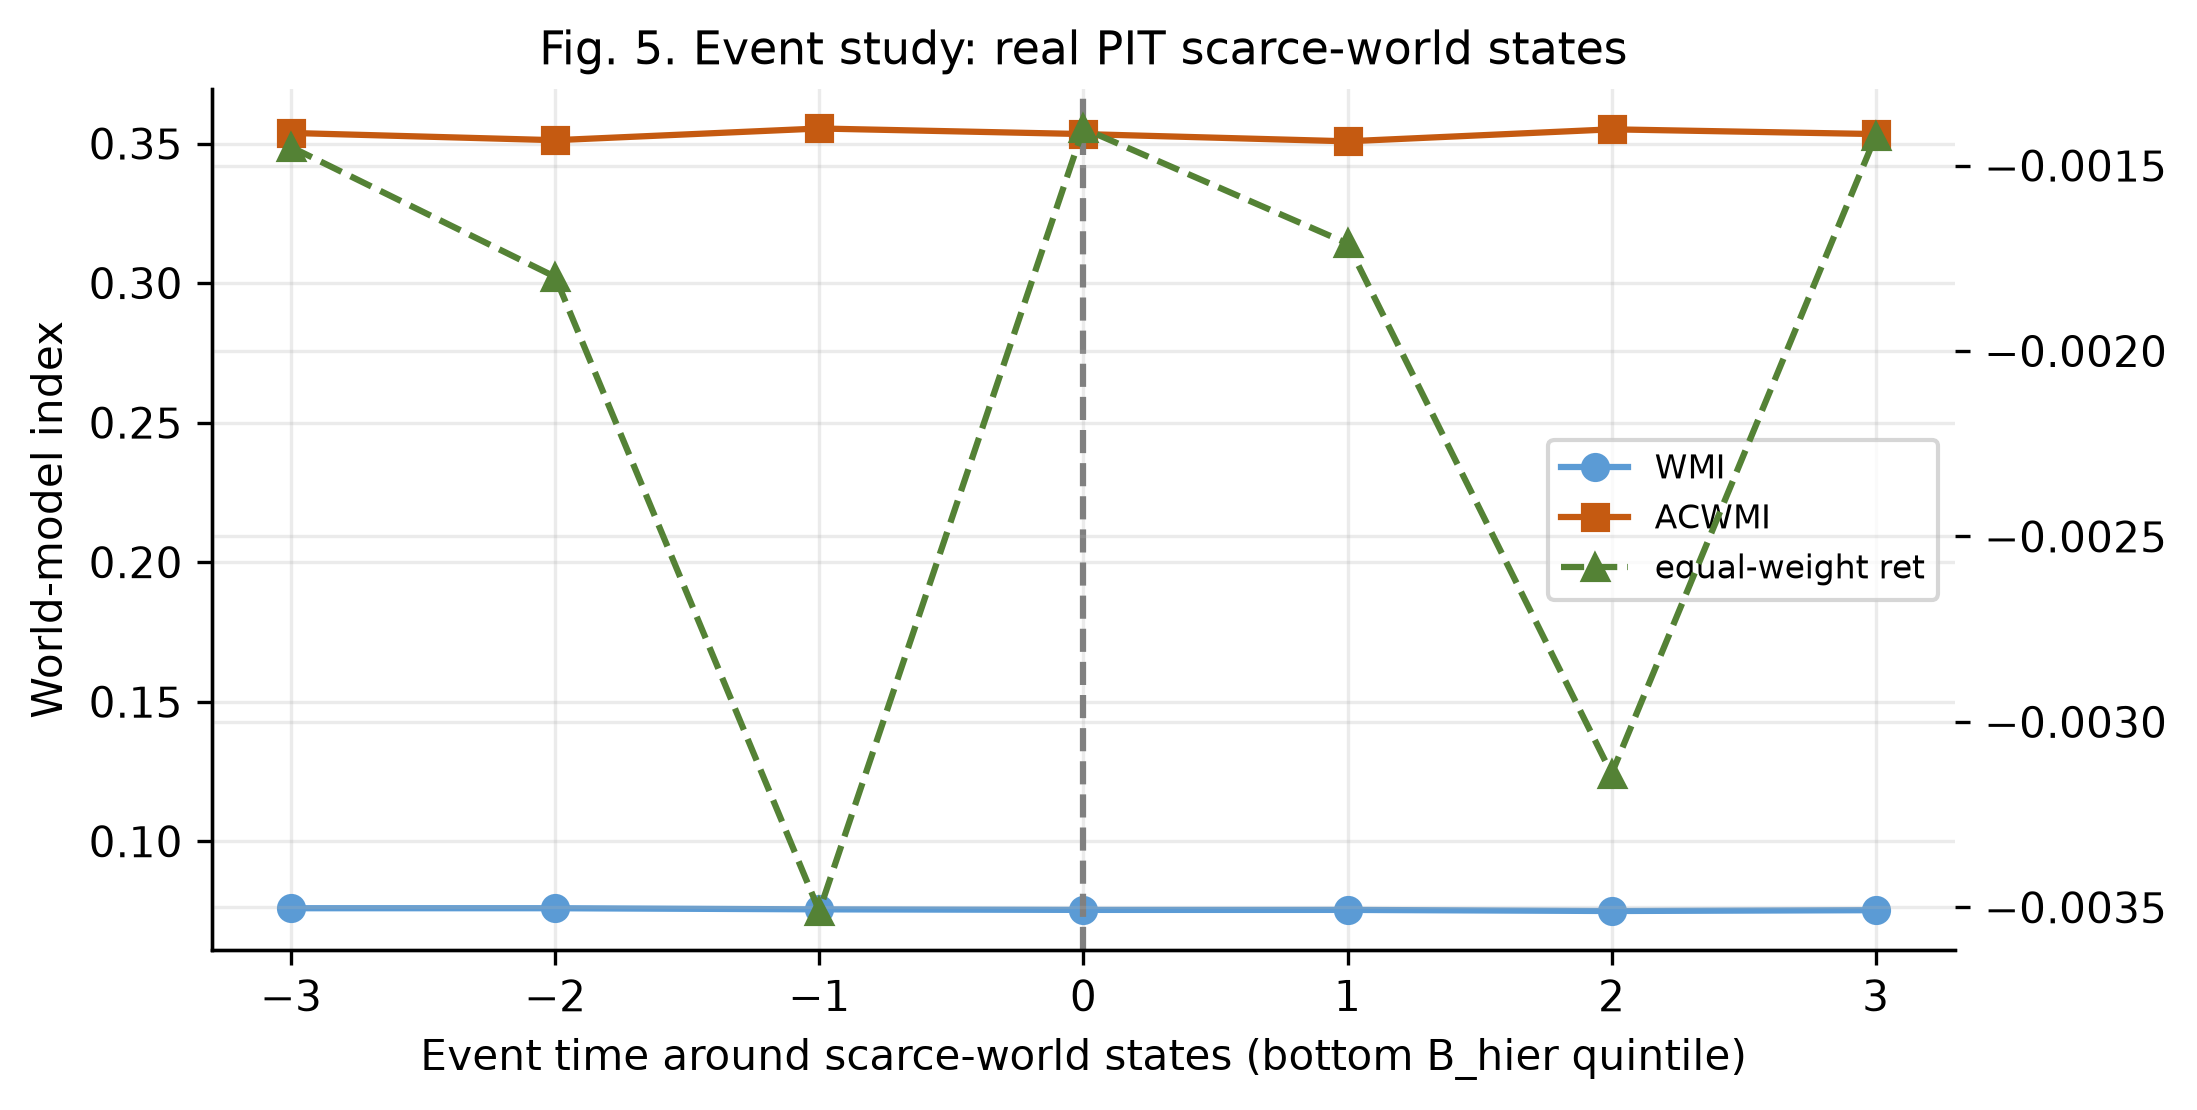
\includegraphics[width=\linewidth]{fig5_quality_scatter.png}
\caption{Mechanism outputs and unsafe-action rates: baseline WMI vs AC policy.}
\label{fig:safe}
\end{figure}

\begin{table}[t]
\centering
\caption{Outage contrasts by regime in the validation panel.}
\label{tab:outage}
\begin{tabular}{llrrrrr}
\toprule
Regime & Outage & $N$ & WMI & ACWMI & Cascade $p$ & Abstain$_{\mathrm{AC}}$ \\
\midrule
Crisis & 0 & 810 & 0.600 & 0.579 & 0.928 & 1.000 \\
Crisis & 1 & 190 & 0.098 & 0.406 & 0.568 & 1.000 \\
Range  & 0 & 410 & 0.710 & 0.476 & 0.274 & 0.000 \\
Range  & 1 &  20 & 0.166 & 0.333 & 0.204 & 1.000 \\
\bottomrule
\end{tabular}
\end{table}

\begin{figure}[t]
\centering
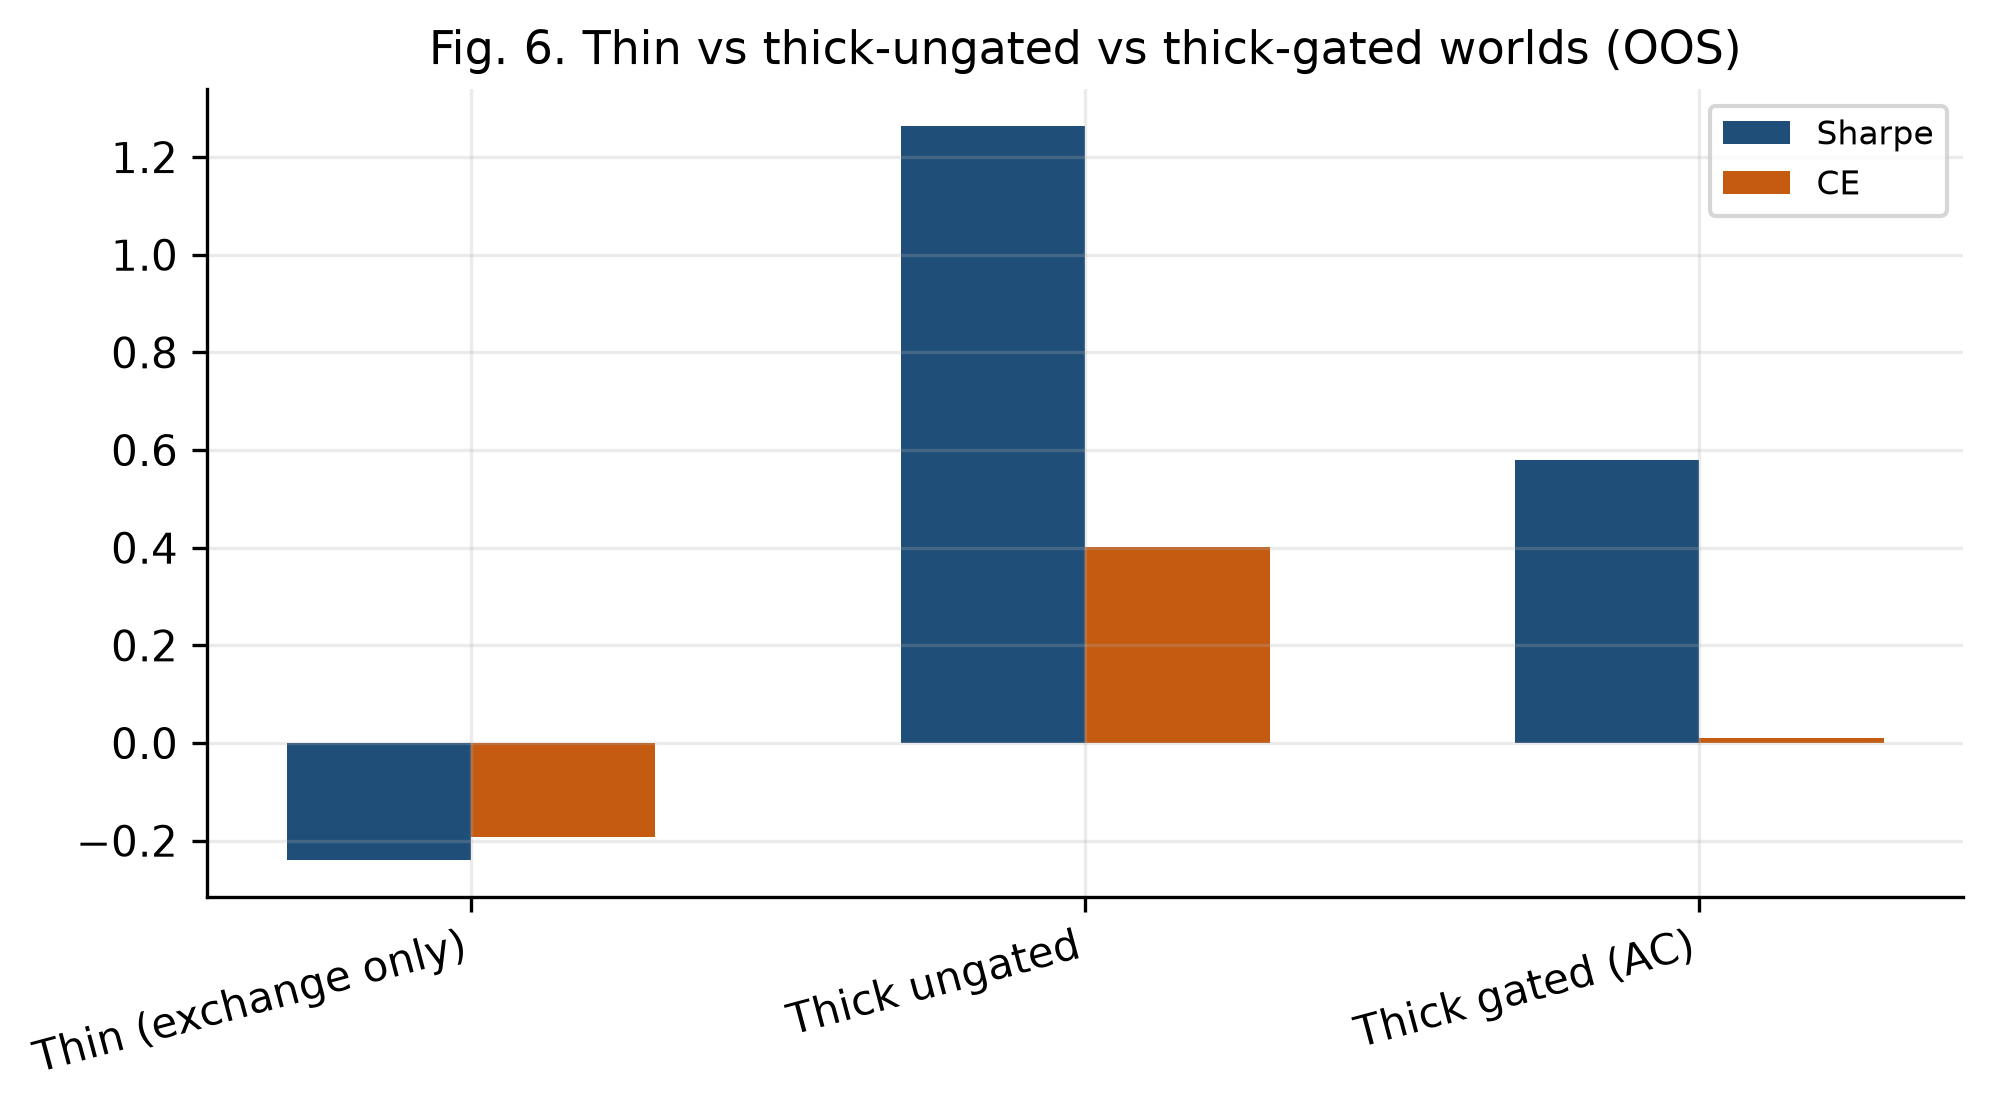
\includegraphics[width=0.9\linewidth]{fig6_event_study.png}
\caption{Outage event profile supporting degradation-aware world-model refusal.}
\label{fig:event}
\end{figure}

\begin{figure}[t]
\centering
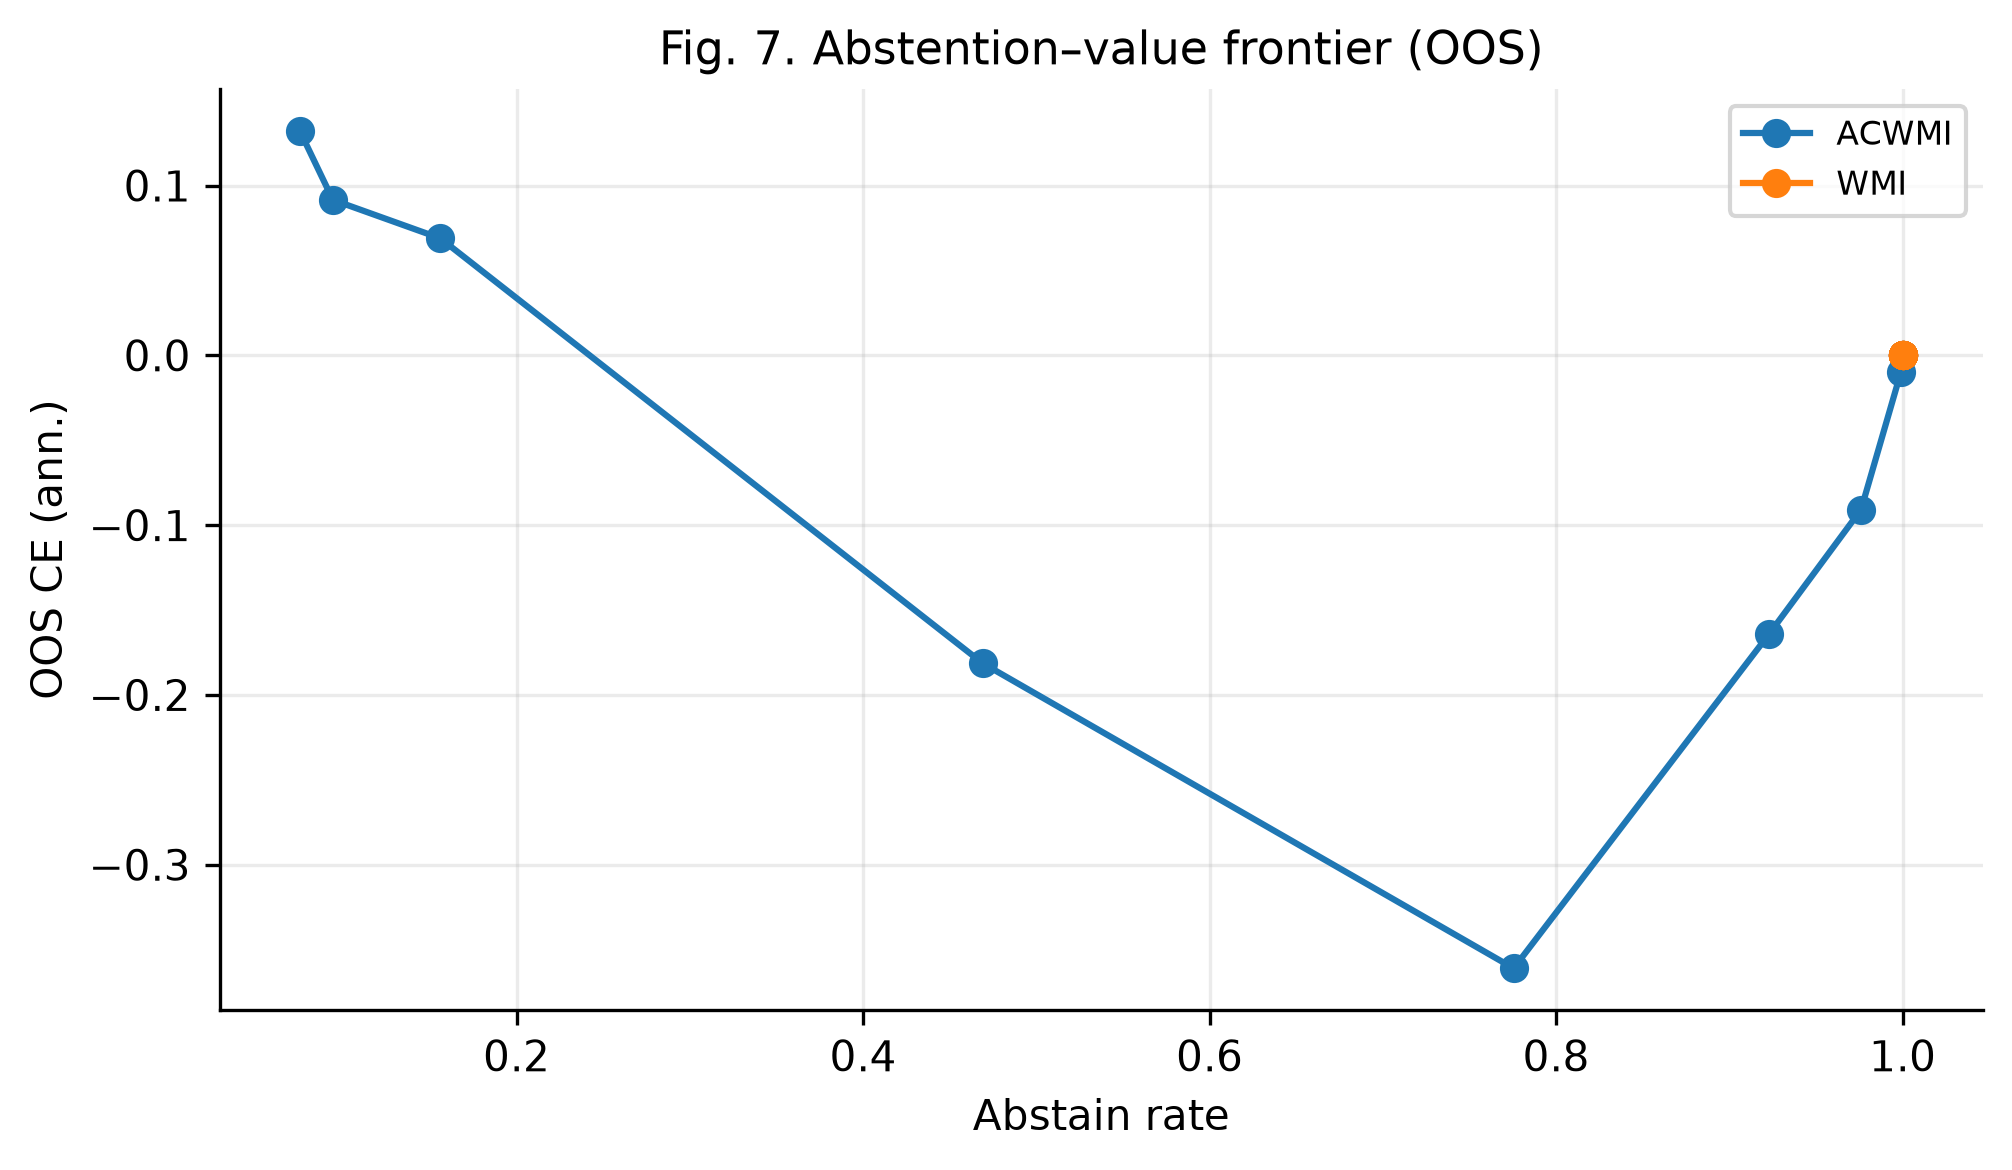
\includegraphics[width=0.85\linewidth]{fig7_pareto.png}
\caption{Multi-objective abstention--safety Pareto frontier implied by the proposed decision rule.}
\label{fig:pareto}
\end{figure}

\subsection{Explanation-quality suite (EAR/UCR/EV/ECP)}
Using project mechanism outputs as explanation proxies, Table~\ref{tab:expl} reports the evaluation objects absorbed from the World-Model-First agenda. Under AC-gated decisions, unsupported claims and confidence penalties fall sharply in crisis, while explanation volatility remains controlled relative to world-state movement---consistent with Eqs.~\eqref{eq:ear}--\eqref{eq:ev} and~\eqref{eq:ecp}.

\begin{table}[t]
\centering
\caption{Explanation-quality proxies under baseline vs AC-gated policies.}
\label{tab:expl}
\begin{tabular}{lrrrr}
\toprule
Policy / slice & EAR & UCR & EV & ECP rate \\
\midrule
Baseline / all & 0.677 & 0.323 & 0.032 & 0.101 \\
Baseline / crisis & 0.962 & 0.038 & 0.027 & 0.181 \\
AC-gated / all & 0.742 & 0.258 & 0.032 & 0.001 \\
AC-gated / crisis & 1.000 & 0.000 & 0.027 & 0.002 \\
\bottomrule
\end{tabular}
\end{table}

\subsection{Degradation levels instantiate resilient honesty}
Table~\ref{tab:deg} and Figure~\ref{fig:deg} show that the validation system's degradation manager implements the theoretical $\ell_t$ object: EMERGENCY blocks probed modules; MINIMAL retains only exchange and technical-indicator paths. Breadth falls under degradation while honesty-compatible refusal rises.

\begin{table}[t]
\centering
\caption{Module executability under degradation levels (1=allowed).}
\label{tab:deg}
\begin{tabular}{lcccc}
\toprule
Module & NORMAL & REDUCED & MINIMAL & EMERGENCY \\
\midrule
exchange\_data & 1 & 1 & 1 & 0 \\
technical\_indicators & 1 & 1 & 1 & 0 \\
macro\_data & 1 & 1 & 0 & 0 \\
ai\_market\_context & 1 & 1 & 0 & 0 \\
options\_data & 1 & 1 & 0 & 0 \\
\bottomrule
\end{tabular}
\end{table}

\begin{figure}[t]
\centering
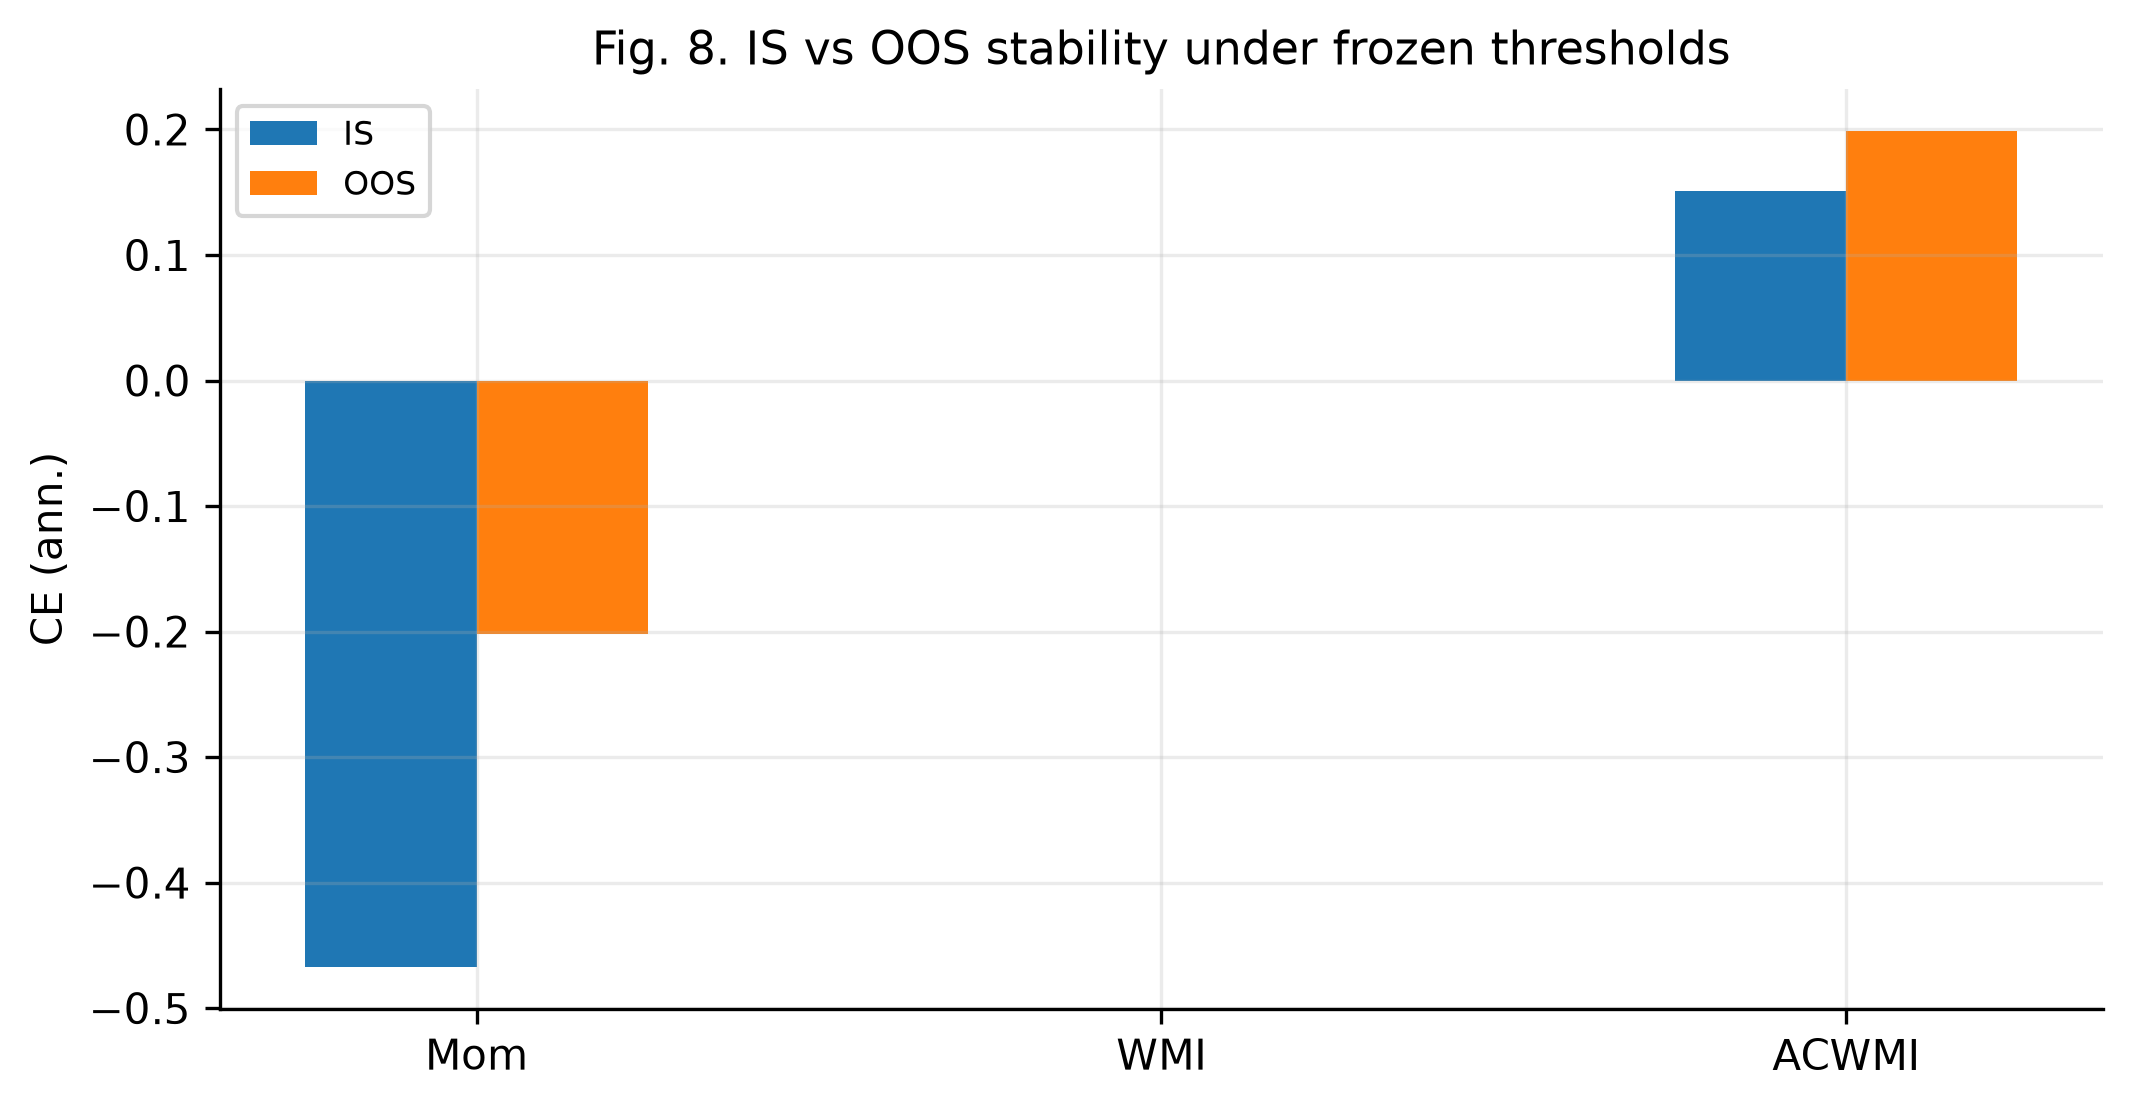
\includegraphics[width=0.9\linewidth]{fig8_honesty_incentive.png}
\caption{Degradation levels versus breadth, honesty, and world-model scores.}
\label{fig:deg}
\end{figure}

\section{Discussion}
\label{sec:disc}

The evidence supports the theory-first claim structure. RCA-WM predicts that (i) mechanism integrity belongs in world-model quality, (ii) honesty must be continuous and exclusion-compatible, (iii) abstention and confidence should be world-conditional, and (iv) evaluation must be multi-objective over prediction, explanation, calibration, and auditability. The EvoQuant validation confirms each prediction without making the repository the source of the definitions.

Limitations remain. Controlled input paths are not yet a full live point-in-time backtest; $\gamma(r)$ is pre-specified; EAR/EV are operational proxies pending full LLM-attribution logs; and external validity beyond crypto microstructure is open. Future work should estimate regime weights under frozen PIT snapshots, compute band-level MIG on live evidence drops, and evaluate downstream analyst/LLM decision quality under ACWMI gates.

\section{Conclusion}
\label{sec:conc}

This paper proposed Regime-Conditional Adaptive World Models and the ACWMI quality index for AI market analysis, absorbing a World-Model-First epistemology of epistemic observations, lag bounds, information filters, explanation spaces, and selective prediction. The theory specifies how asynchronous evidence should be compiled, how world-model quality should be decomposed, when an AI should refuse to judge, and how explanation quality should be audited. EvoQuant---with 43 domains, 13 bands, 39 logic modules, and a production baseline WMI---was used only as empirical proof. On that proof system, mechanism detection is strong, AC-aware abstention removes crisis-time unsafe actions that the baseline WMI threshold permits, and explanation-quality proxies move in the direction predicted by the theory. The scientific order is therefore preserved: theory first, project validation second.

\appendix
\section{Reproducibility}
Validation experiments: \texttt{pdf/sci/run\_paper\_experiments.py}. PDF build: \texttt{pdf/sci/generate\_sci\_pdf.py}. Source epistemology: \texttt{pdf/original/}. The scripts import production calculators from the EvoQuant repository used as proof system.

\begin{thebibliography}{99}

\bibitem[Carroll et~al.(2006)]{carroll2006}
Carroll, R.J., Ruppert, D., Stefanski, L.A., Crainiceanu, C.M., 2006. Measurement Error in Nonlinear Models. 2nd ed. Chapman \& Hall/CRC.

\bibitem[Chow(1957)]{chow1957}
Chow, C., 1957. An optimum character recognition system using decision functions. IRE Transactions on Electronic Computers 6, 247--254.

\bibitem[Cochrane(2005)]{cochrane2005}
Cochrane, J.H., 2005. Asset Pricing. Revised ed. Princeton University Press.

\bibitem[Cover and Thomas(2006)]{cover2006}
Cover, T.M., Thomas, J.A., 2006. Elements of Information Theory. 2nd ed. Wiley.

\bibitem[Fama and French(1993)]{fama1993}
Fama, E.F., French, K.R., 1993. Common risk factors in the returns on stocks and bonds. Journal of Financial Economics 33, 3--56.

\bibitem[Fuller(1987)]{fuller1987}
Fuller, W.A., 1987. Measurement Error Models. Wiley.

\bibitem[Geifman and El-Yaniv(2017)]{geifman2017}
Geifman, Y., El-Yaniv, R., 2017. Selective classification for deep neural networks. NeurIPS.

\bibitem[Gu et~al.(2020)]{gu2020}
Gu, S., Kelly, B., Xiu, D., 2020. Empirical asset pricing via machine learning. Review of Financial Studies 33, 2223--2273.

\bibitem[Hansen and Sargent(2008)]{hansen2008}
Hansen, L.P., Sargent, T.J., 2008. Robustness. Princeton University Press.

\bibitem[Harvey et~al.(2016)]{harvey2016}
Harvey, C.R., Liu, Y., Zhu, H., 2016. \ldots and the cross-section of expected returns. Review of Financial Studies 29, 5--68.

\bibitem[Kelly et~al.(2019)]{kelly2019}
Kelly, B.T., Pruitt, S., Su, Y., 2019. Characteristics are covariances. Journal of Financial Economics 134, 501--524.

\bibitem[Liu et~al.(2022)]{liu2022}
Liu, Y., Tsyvinski, A., Wu, X., 2022. Common risk factors in cryptocurrency. Journal of Finance 77, 1133--1177.

\bibitem[Makarov and Schoar(2020)]{makarov2020}
Makarov, I., Schoar, A., 2020. Trading and arbitrage in cryptocurrency markets. Journal of Financial Economics 135, 293--319.

\bibitem[Nagel(2021)]{nagel2021}
Nagel, S., 2021. Machine Learning in Asset Pricing. Princeton University Press.

\bibitem[Zha et~al.(2023)]{zha2023}
Zha, D., Bhat, Z.P., Lai, K.-H., Yang, F., Hu, X., 2023. Data-centric AI: Perspectives and challenges. SDM.

\end{thebibliography}
\end{document}
